\documentclass[letterpaper, 10 pt, conference]{ieeeconf}  % Comment this line out if you need a4paper

%\documentclass[a4paper, 10pt, conference]{ieeeconf}      % Use this line for a4 paper

\IEEEoverridecommandlockouts                              % This command is only needed if 
                                                          % you want to use the \thanks command

\overrideIEEEmargins                                      % Needed to meet printer requirements.

% See the \addtolength command later in the file to balance the column lengths
% on the last page of the document

% The following packages can be found on http:\\www.ctan.org
\usepackage{graphicx} % for pdf, bitmapped graphics files
\graphicspath{{../}}
\usepackage{epstopdf} % for postscript graphics files
\usepackage{mathptmx} % assumes new font selection scheme installed
\usepackage{times} % assumes new font selection scheme installed
\usepackage{amsmath} % assumes amsmath package installed
\usepackage{amssymb}  % assumes amsmath package installed
\usepackage[caption=false,font=footnotesize]{subfig}
\usepackage{fixltx2e}
\usepackage{float}

\title{\LARGE \bf
3D-PIV application for autonomous vehicles using monocular vision
}


\author{Eduardo Afonso$^{1}$ and Researcher$^{2}$% <-this % stops a space
\thanks{$^{1}$ Eduardo Afonso is coursing Control and Automation Engineering,
        Federal University of Lavras, Lavras - MG, Brazil.
        {\tt\small eduardo.afonso@engautomacao.ufla.br}}%
\thanks{$^{2}$ Researcheris with the Department of Electrical Engineering, Wright State University,
        Dayton, OH 45435, USA
        {\tt\small b.d.researcher@ieee.org}}%
}


\begin{document}


\maketitle
\thispagestyle{empty}
\pagestyle{empty}

\begin{abstract}


\end{abstract}

\section{INTRODUCTION}

Monocular vision has been demonstrating a flourishing field in autonomous vehicles. Several applications have presented  
solutions to current problems. Although systems of low computational cost and effectivity are a challenge to field. \\
The Particle Image Velocimetry (PIV)\cite{Bastiaans} is used in many fields of knowledge \cite{Story, Xu}, to calculate 
the velocity of fluids in different parts. Here, PIV was adjusted for situation of autonomous vehicles, using PCC
\cite{Miranda Neto} and KITTI's bank of dates\cite{Geiger}.\\

\section{THEORETICAL FUNDAMENT}

\subsection{PEARSON CORRELATION COEFFICIENT - PCC}

PCC is used in statistical analyses, pattern recognition and computer vision. 
Applications include disparity measurement and object recognition, comparing two images. The followed equation
describes PCC for monochrome digital images\cite{Eugene}:

\begin{equation}$$
\centering
\everymath{\displaystyle}
$r_i = \frac{\sum\limits_i (x_i-x_m)(y_i-y_m)}{\sqrt{\sum\limits_i (x_i-x_m)^2} \sqrt{\sum\limits_i (y_i-y_m)^2}}
$
$$\end{equation}

Where, $x_i$ is the intensity of the i-th pixel in image 1, $y_i$ is the intensity of the i-th pixel in image 2, $x_m$ is 
the mean intensity of image 1, and $y_m$ is the mean intensity of image 2 \cite{Miranda Neto}.

\subsection{PARTICLE IMAGE VELOCIMETRY - PIV}

PIV is a method to determine a velocity field from images of seeded flows\cite{Bastiaans}.
Its result is given as as field of vectors, demonstrating direction, sense and intensity of velocity in each particle. Moreover,
it is possible to calculate rapidly the velocities of any part of image.\\

\section{SYSTEM DESCRIPTION}
The purpose of this algorithm is tracking objects, producing added informations about the followed target.
The algorithm developed takes as inputs sequential frames and Region Of Interesting(ROI). They are important to
define the parameters used to generate the tracking of objects and other details as: the relative velocity, the factor of 
approaching and of departure

With ROI determined, the system enters in looping to follow the target as shown in the fig. 1.

\begin{figure}[bhp]
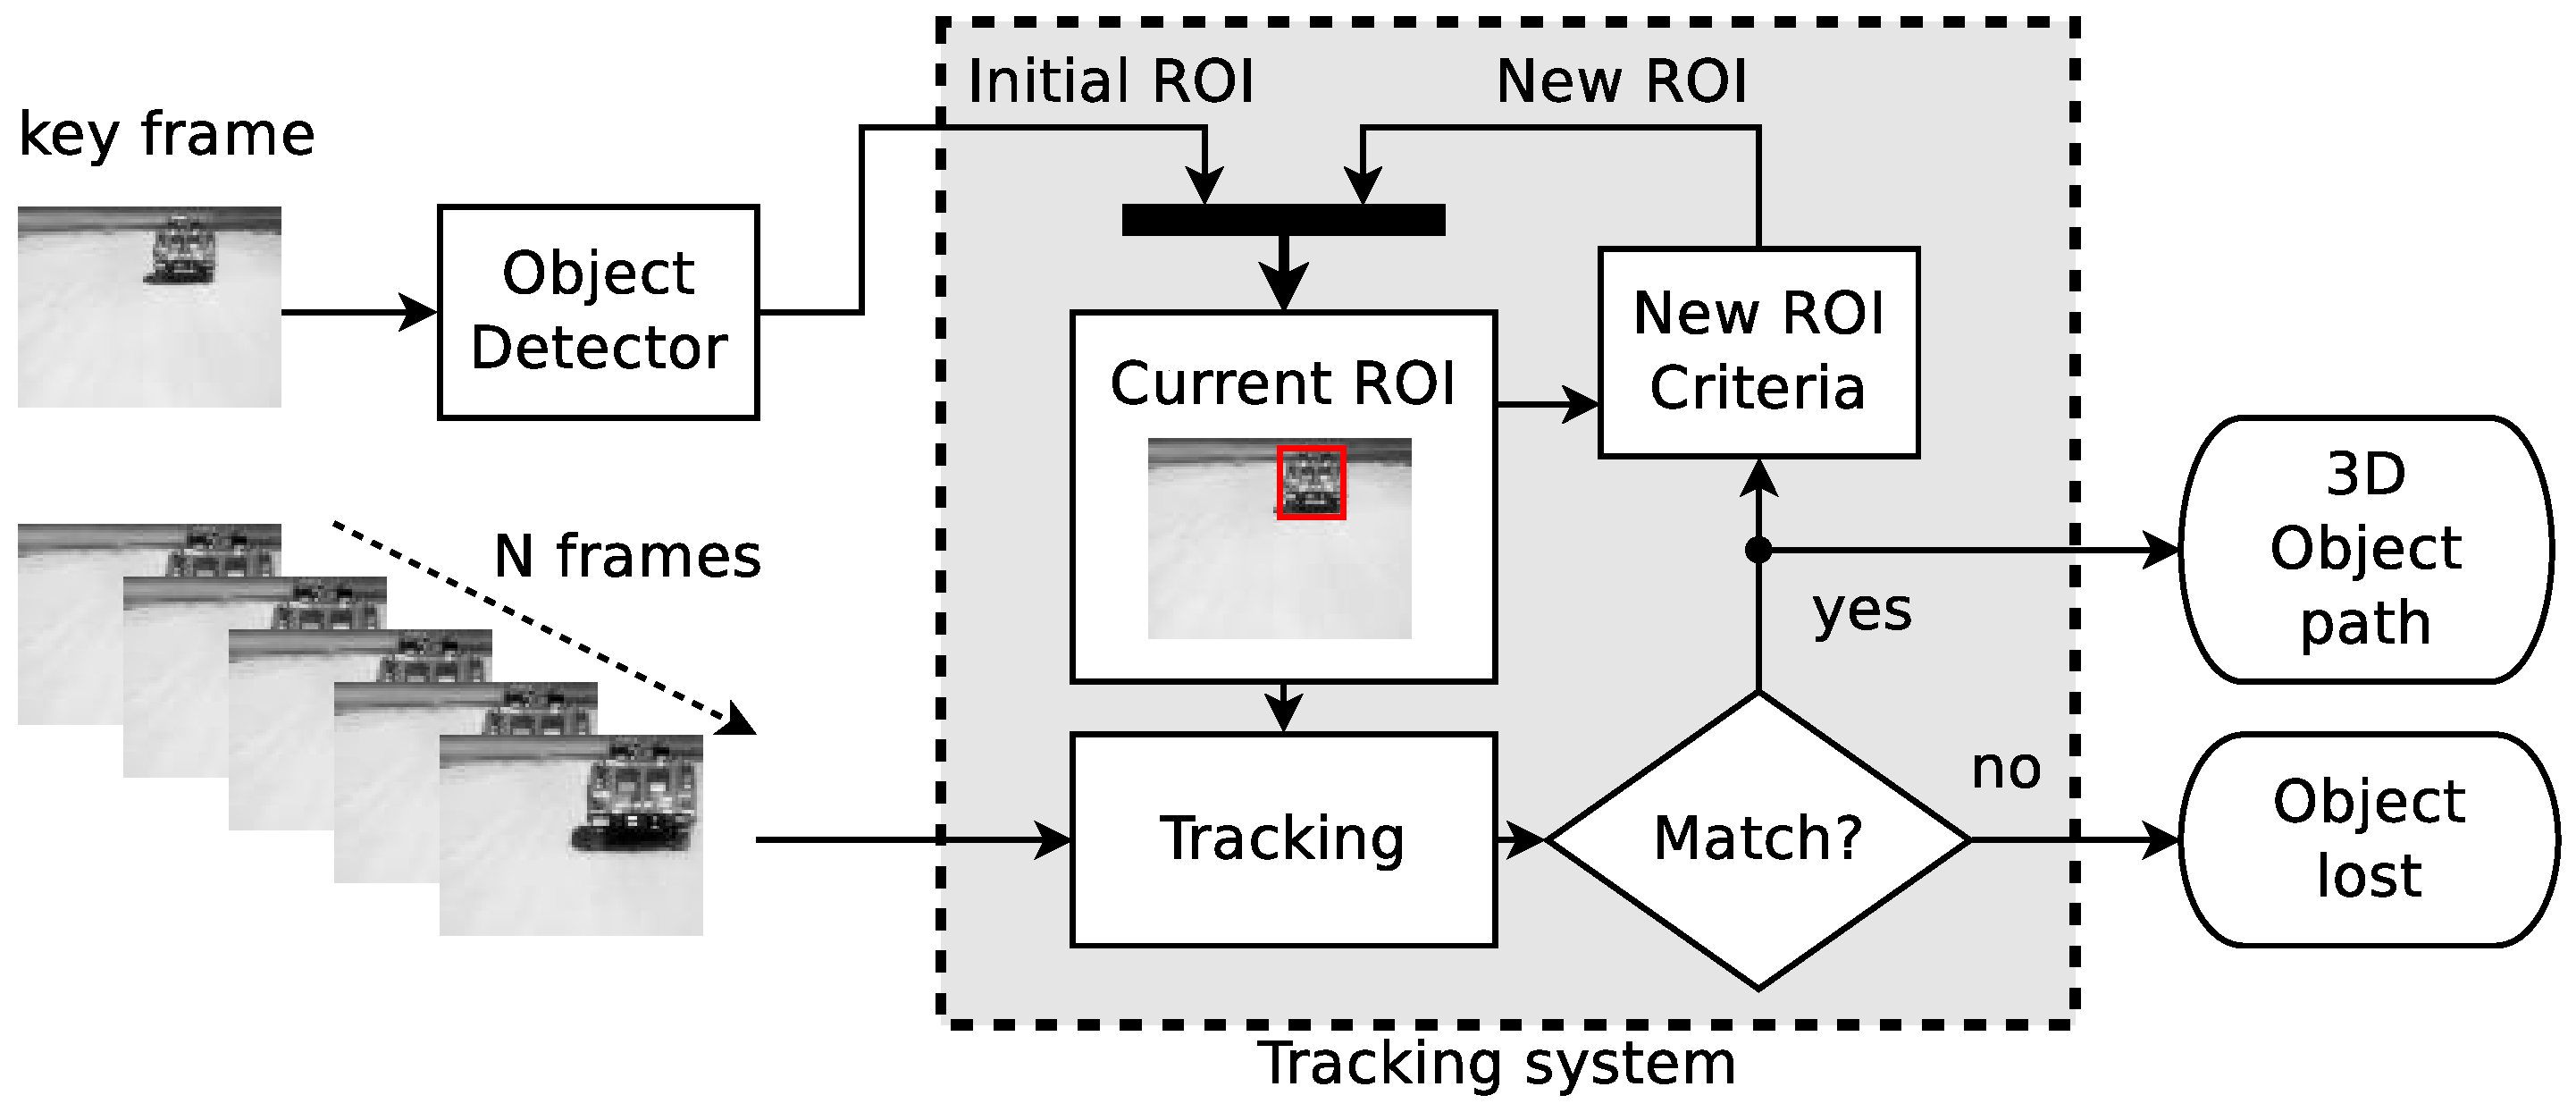
\includegraphics[width=\columnwidth]{images/figure1-diagram1.eps}
\caption{With object detected, the highest value of PCC in the Window Of Search (WOS) of next frame identifies the target, 
and the result of search is a vector. 
Which its beginning and its end are on the first and last position, respectively. After, these processing is made again for 
next frames.}
\end{figure}

In 2 dimensions, the objects are tracking and given information about its horizontal or vertical relative velocity.
When the target moves in 3 dimensions, outputs are the resultant of relative velocity and the factor of approaching or departure. 
There isn't a factor in 2 dimensions, since approaching or departure don't exist in this situation.

%Diagrama1
 %A gente vai explicar o algoritmo como uma caixa fechada , que coisa entra e que coisa sai
 %e os parametros a sintonizar.
 % como usar ele quando implementado, como se fosse uma caixa preta.
 
\section{ALGORITHM DESCRIPTION}
 
%DiagramaX

\subsection{MULTI-RESOLUTION MATCH CRITERIA}
Method to track object at image is based on PIV. Figure 2(a) shows the application in 2 dimensions and the next in
3 dimensions.

\begin{figure}[H]
\centering
  \subfloat[]{\label{subfig:(a)} 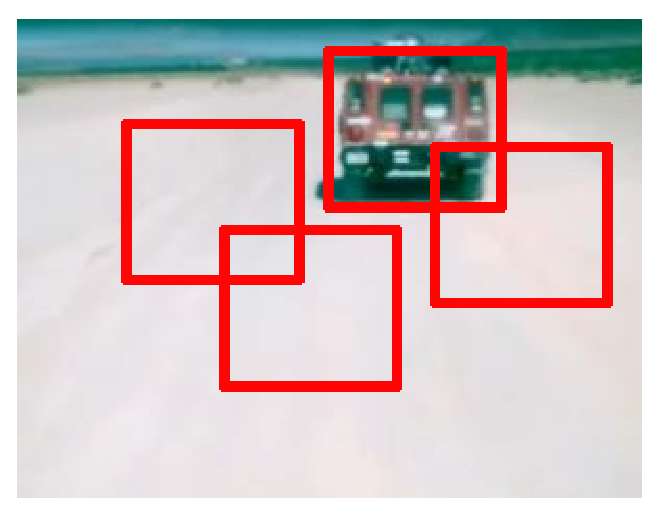
\includegraphics[width=.5\columnwidth]{images/figure2a.eps}}
  \subfloat[]{\label{subfig:(b)} 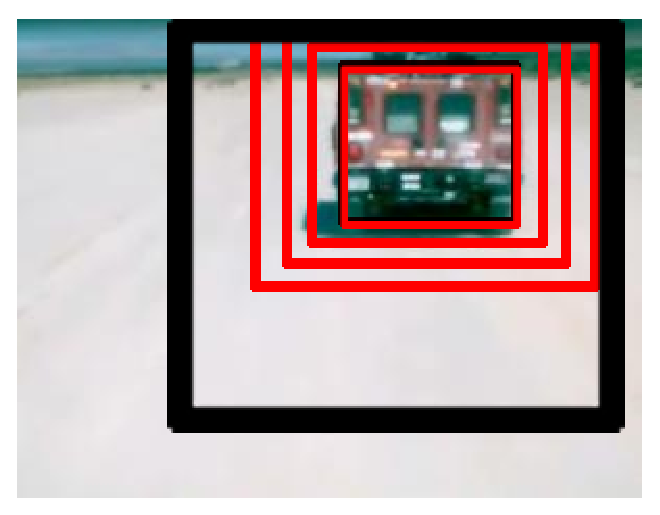
\includegraphics[width=.5\columnwidth]{images/figure2b.eps}}
  \caption{The red box in figure (a) shows the ROI and black box is WOS. In the figure (a), 
  ROI is compared with first portion on the left top of WOS, and these comparisons are made 
  pixel by pixel for whole WOS. The black boxes, in the figure (b), are the WOS used 
  to different layers of search in 3 dimensions}
\end{figure}

To track the object, the ROI defines the size of WOS and, verify the similarity of ROI and parts of WOS using PCC. 
The highest coefficient of Pearson determines new place of object. The figure 2(b) reveals how the dimension of depth was included and, 
the search is made in different layers. In 3 dimensions, the target also is found from the highest PCC among WOS, but the object may be 
bigger or smaller, depending in which layers was.\\
%onde estava, onde esta agora
%que tamanho tinha que tamanho tem.
\subsubsection{MULTI-LAYER 3D APPROXIMATION}
The multi-layer is a technique to track objects that move in 3 dimensions. The layers are organized of the smallest to the biggest, 
there is a rate which layers increase. With this proceeding, the algorithm is capable of track objects that in second scene was larger than first.\\

%usa Multi-resolution match criteria e explica isso dos tamanhos

\subsubsection{FACTOR OF APPROACHING - RELATIVE VELOCITY}
Factor of approaching is a dimensionless number related to the rate of approaching or departure of an object to the camera. The factor
is determined how showed at equation 2:

\begin{equation}
\centering
\everymath{\displaystyle}
f_a = \frac{Area_r}{Area_f} 
\end{equation}

Where $f_a$ is the factor of approaching, $Area_r$ is area of ROI and $Area_f$ is area of current frame.\\
The factor has two means, e.g., if the rate of approaching increase quickly, so the target is approaching. Or the apposite, if factor decreases, thus 
object is departing.\\
Relative velocity is calculate using a simples equation of kinematic in physics:


\begin{equation}
\centering
\everymath{\displaystyle}
 v = \frac{\Delta s}{\Delta t}
\end{equation}

Where $v$ is relative velocity, $\Delta s$ is difference in between two pixels and $\Delta t$ is time of proceeding.\\
Velocity calculated is relative for simple reason that it is impossible to know the real distance between the camera and object in this
condition.\\

\subsection{RENEW ROI CRITERIA}
%Diagrama2
Region of Interesting is an important element of algorithm because this decides what will be found at image. The mean question in this case is 
the best moment to change ROI. When the comparison of images reaches the threshold 0.925, then ROI is changed. The threshold adopted is 0.8 to 
match case\cite{Eugene}.


\begin{figure}[H]
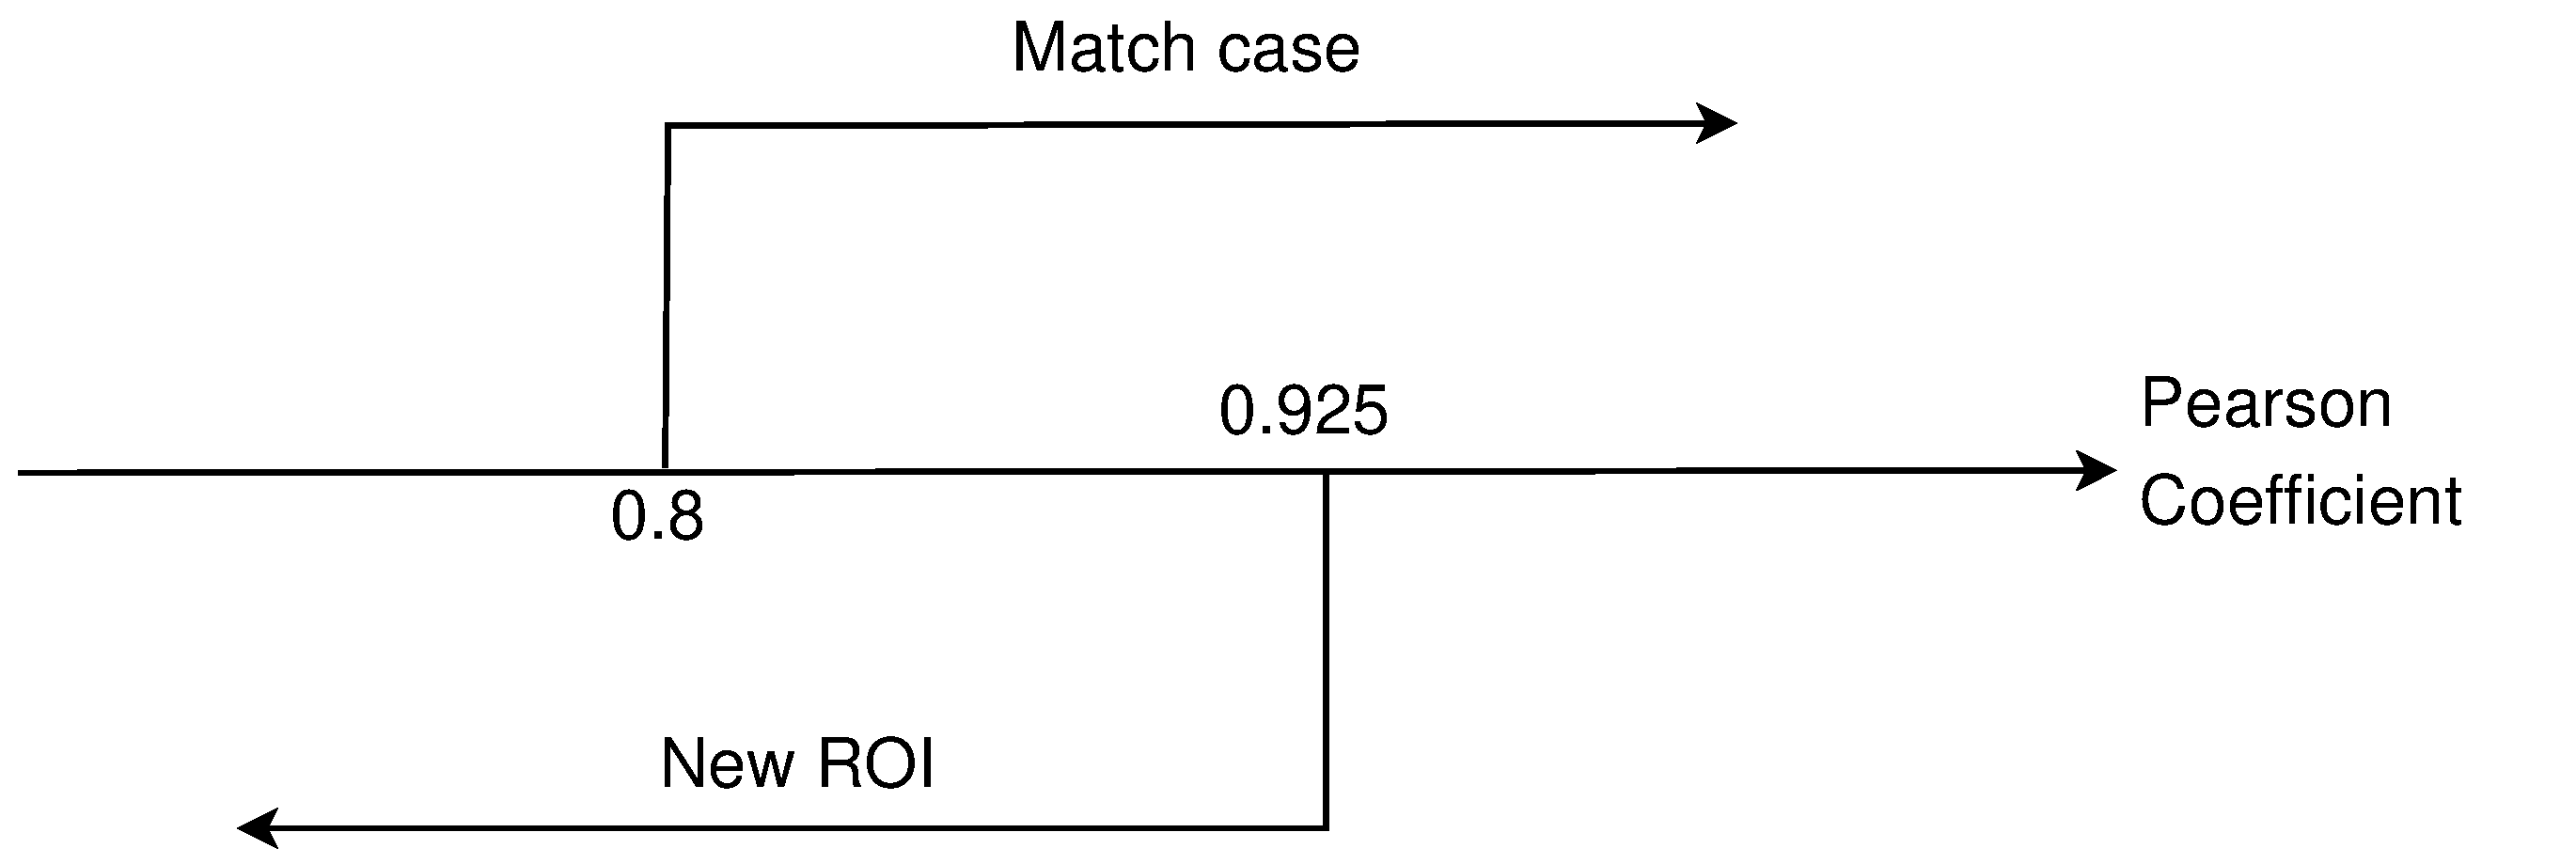
\includegraphics[width=\columnwidth]{images/figure3.eps}
\caption{When the comparison is more than 0.8, including numbers bigger than 0.925, the target was matched. But if two images are compared 
and PCC is less than 0.925, so the ROI changes to the last ROI compared.}
\end{figure}

The system needs to have high level of reliability, so the threshold adopted contributes to an operation with minimum of mistakes.

% descri��o do sistemA
\section{NUMERICAL RESULTS}
%testes com diferentes parametros
% tabelas e graficos

\section{CONCLUSIONS}

PIV has presented satisfactory results. Different kinds of information that can be concluded, like: estimate collision, tracking of
objects in 2 or 3 dimensions and factor of approaching and removal. The simulations in Matlab has given promissories results.

\addtolength{\textheight}{-12cm}

\section*{ACKNOWLEDGMENT}

%FAPEMIG\\
%numero de bolsa\\
%numero de projeto\\
%numero de aluno


\begin{thebibliography}{99}

\bibitem{Auoude} G.S. Auoude et al. Sampling-Based Threat Assessment Algorithms for Intersection Collisions Involving 
        Errant Drivers. IFAC Symposium on Intelligent Autonomous Vehicles, 2010.
        
	\bibitem{Bastiaans} R. J. M. Bastiaans, Cross-correlation PIV; theory, implementation and accuracy. 
        Eindhoven: Technische Universiteit Eindhoven, 2000. - EUT Report 99-W-OOl. - ISBN: 90-386-2851-X.
        
        \bibitem{Eugene} Y. K. Eugene and R.G. Johnston, The Ineffectiveness of the Correlation Coefficient for Image Comparisons.
        Technical Report LA-UR-96-2474, Los Alamos, 1996.
        
        \bibitem{Geiger} A. Geiger et al,
        Vision meets Robotics: The KITTI Dataset. International Journal of Robotics Research (IJRR), 2013.
        
        \bibitem{Jonas} T. Jonas, Real-Time Probabilistic Collision Avoidance for Autonomous Vehicles, Using Order Reductive 
        Conflict Metrics. Submitted to the Department of Aeronautics and Astronautics
	in partial fulfillment of the requirements for the degree of Doctor of Philosophy. Massachusetts Institute of Technology. June, 2003.
        
        \bibitem{Miranda Neto} A. Miranda Neto et al, Image Processing Using Pearson's Correlation Coefficient: 
        Applications on Autonomous Robotics. 
        Autonomous Robot Systems (Robotica), 2013 13th International Conference on, 2013.
	
	\bibitem{Story} A. Story et al, PIV measurements of the velocity field of a Newtonian Fluid in a stirred tank equipped 
	with the PMT type impeller.Technical Transactions - Chemistry. 2-Ch/2014.
	
	\bibitem{Woerner} K. Woerner, COLREGS-Compliant Autonomous Collision Avoidance Using Multi-Objective Optimization
	with Interval Programming. Submitted to the Department of Mechanical Engineering in partial fulfillment of the requirements for the 
	degrees of Naval Engineer and Master of Science in Mechanical Engineering. Massachusetts Institute of Technology. June, 2014.
	
	\bibitem{Xu} L. Xu, Computational fluid dynamics analysis and PIV validation of a bionic vortex flow 
	pulsatile LVAD.Technology and Health Care 23 (2015) S443?S451. DOI 10.3233/THC-150981. IOS Press, 2015.


\end{thebibliography}

\end{document}
